

\section{Introduction}
The prevalence of positioning devices has drastically boosted 
the scale and spectrum of trajectory collection to an unprecedented level. 
Tremendous amounts of trajectories, in the form of sequenced spatial-temporal 
records, are continually generated from animal telemetry chips, 
vehicle GPSs and wearable devices. Data analysis on large-scale 
trajectories benefits a wide range of applications and services, 
including traffic planning~\cite{zheng2011urban}, animal analysis~\cite{li2010miningperiodic}, and social recommendations~\cite{bao2013survey}, to name just a few.


A crucial task of data analysis on top of trajectories is 
to discover co-moving patterns. A \emph{co-movement} pattern~\cite{li2013managing} 
refers to a group of objects traveling together for a certain period of time 
and the group is normally determined by spatial proximity. 
A pattern is prominent if the size of the group exceeds $M$ and the length of the duration exceeds $K$, where $M$ and $K$ are parameters specified by users. Rooted from such basic definition 
and driven by different mining applications, there are a bunch of variants 
of co-movement patterns that have been developed with more advanced constraints.

Table~\ref{tbl:existing_co_patterns} summarizes several popular co-moving patterns 
with different constraints in the attributes of clustering in spatial proximity,
consecutiveness in temporal duration and computational complexity. 
In particular,  the \emph{flock}~\cite{gudmundsson2006flock} 
and \emph{group}~\cite{wang2006grouppattern} patterns require 
all the objects in a group to be enclosed by a disk with radius $r$; 
whereas the \emph{convoy}~\cite{jeung2008convoy}, \emph{swarm}~\cite{li2010swarm} 
and \emph{platoon}~\cite{li2015platoon} patterns resort to density-based 
spatial clustering. 
In the temporal dimension, \emph{flock}~\cite{gudmundsson2006flock} 
and \emph{convoy}~\cite{jeung2008convoy} require all the timestamps 
of each detected spatial group to be consecutive, which is referred to as \emph{global consecutiveness}; 
whereas \emph{swarm}~\cite{li2010swarm} does not impose any restriction. 
The \emph{group}~\cite{wang2006grouppattern} and \emph{platoon}~\cite{li2015platoon} adopt a compromised manner by allowing
arbitrary gaps between the consecutive segments, which is called \emph{local consecutiveness}. 
They introduce a parameter $L$ to control the minimum length of each local consecutive segment.


%Specifically, a \emph{flock}~\cite{gudmundsson2006flock} requires the group to be within a disk region of
%the user specified size.  A \emph{convoy}~\cite{jeung2008convoy} requires a group to be densely connected. Both \emph{flock}
%and \emph{convoy} require a group to appear for at least $k$ consecutive times.  
%\emph{Group}~\cite{wang2006grouppattern} and 
%\emph{Swarm}~\cite{li2010swarm} patterns relax the consecutiveness constraint, where non-consecutive timestamps are allowed in a pattern duration. \emph{Group} pattern require objects in a group to be within a disk region, while \emph{swarm}require the objects in a group to be densely connected.
%Recently,
%\emph{platoon}~\cite{li2015platoon} pattern is proposed to impose a fine-grained control on the consecutiveness of the duration. In \emph{platoon}, the duration of a group needs to have the local-consecutive portion of size no less than the user-specified $L$.

\begin{table} \scriptsize
\centering
\begin{tabular}{|c|c|c|c|}
\hline 
 & Proximity & Consecutiveness &  Time Complexity\\ 
\hline 
flock~\cite{gudmundsson2004flock} & disk-based &  global & $O(|\mathbb{O}||\mathbb{T}|^2 + |\mathbb{O}|log(|\mathbb{O}|))$ \\ 
\hline 
convoy~\cite{jeung2008convoy} & density-based &   global & $O(|\mathbb{O}|^2+|\mathbb{O}||\mathbb{T}|)$\\ 
\hline 
group~\cite{wang2006grouppattern} & disk-based &  local & $O(|\mathbb{O}|^2|\mathbb{T}|)$ \\ 
\hline 
platoon~\cite{li2015platoon} & density-based &  local & $O(2^{|\mathbb{O}|}|\mathbb{O}||\mathbb{T}|)$\\ 
\hline 
swarm~\cite{li2010swarm} & density-based  & no constraint & $O(2^{|\mathbb{O}|}|\mathbb{O}||\mathbb{T}|)$  \\ 
\hline 
\end{tabular} 
\caption{Constraints and complexity of co-movement patterns. The time complexity indicates the performance in the worst case, where $|\mathbb{O}|$ is the total number of objects and $|\mathbb{T}|$ is the number of descritized timestamps.}
\label{tbl:existing_co_patterns}
\end{table}

%of densely connected objects that travel together for at least $k$ consecutive time. A \emph{swarm}~\cite{li2010swarm} relax the consecutiveness of \emph{convoy}.
% 
%To formally define the pattern, the temporal dimension of trajectories is descritized into snapshots, where each snapshot contains the geographical information of all moving objects. 
%Given a member size constraint $n$, a temporal constraint $k$, a \emph{co-movement} pattern finds a cluster of objects with at least size $n$ and close in spatial proximity for at least $k$ snapshots. 
%Recently, there have been several works extending the basic pattern to incorporate more advanced temporal constraints. For instance, Jeung et al. proposed \emph{convoy} pattern, which requires the snapshots to be consecutive; Li et al. proposed \emph{swarm} pattern, which relaxes the consecutiveness of snapshots and Li et al. proposed \emph{platoon} pattern which imposed a \emph{minimum local length} on the snapshots. 
%PLEASE BE MORE SPECIFIC FOR THE THREE PATTERNS. ALSO, ADD THE CITATIONS.
\begin{figure}[h]
\centering
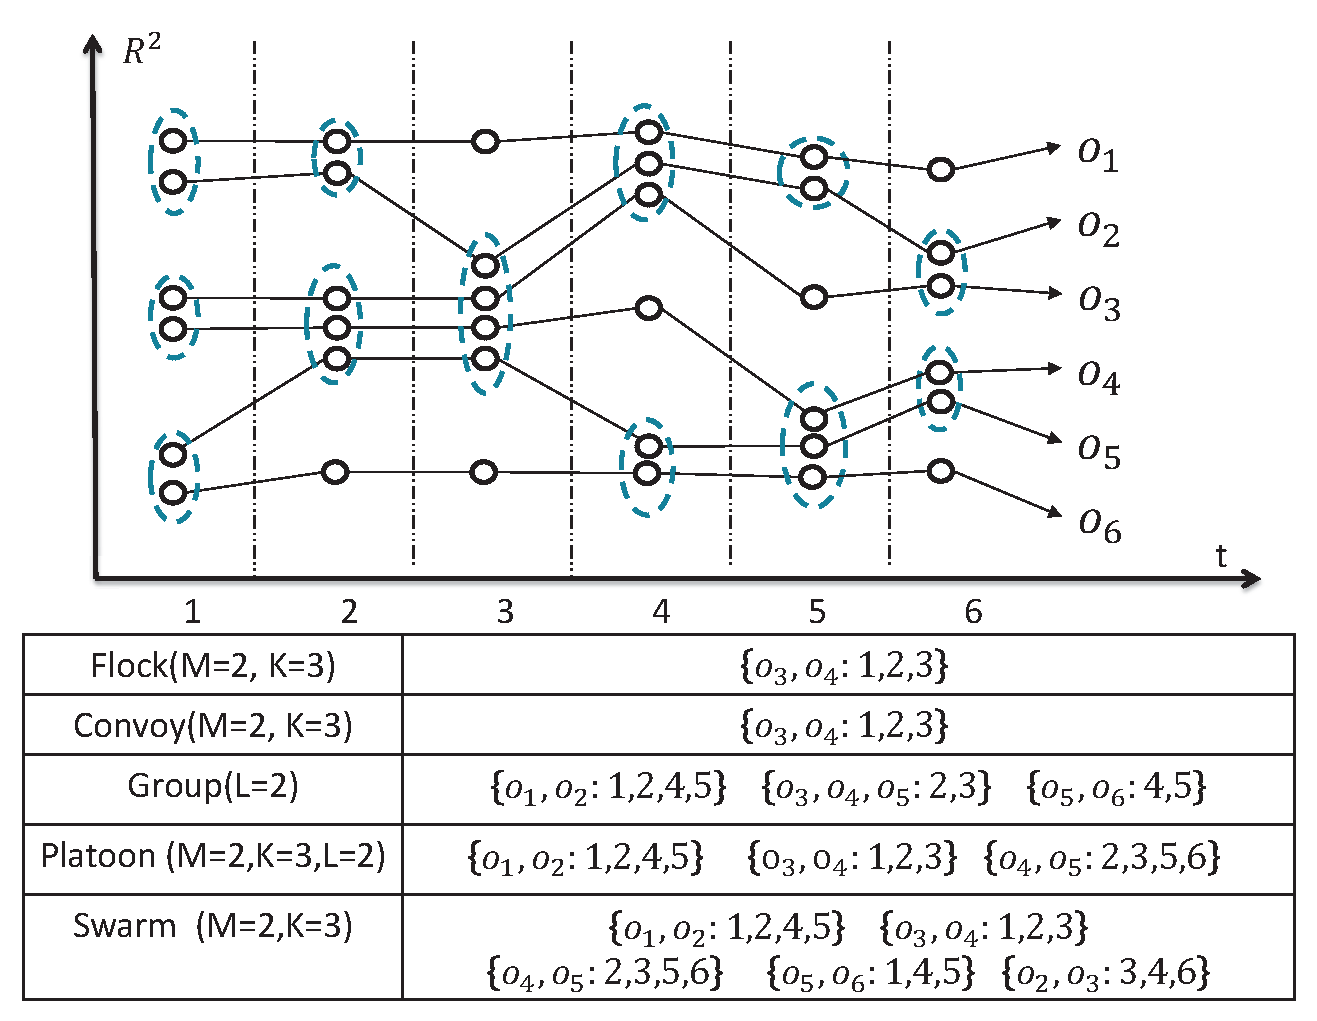
\includegraphics[width=0.45\textwidth]{related_work.eps}
\caption{Trajectories and co-movement patterns; The example consists of six trajectories across six snapshots. The
clusters of objects in each snapshots are denoted using dotted circles. Each type of pattern has its parameters. 
$M$ denotes the minimum size of objects.
$K$ denotes the minimum size of timestamps.
$L$ denotes the minimum size of locally consecutive timestamps.}
\label{fig:related_work}
\end{figure}

%%We first provide a synthetic example to better illustrate these patterns in Figure~\ref{fig:related_work}, and the formal definitions are described in Section~\ref{sec:definition}.
%UPDATE THE FIGURE TO CONTAIN SIX SNAPSHOTS. USE A NEW REPRESENTATION OF THE PATTERN. I DON'T LIKE $\{o_1,o_2\}\{1,2,3\}$. USE ONE PAIR OF $\{\}$ ONLY.

We compare and contrast these patterns using Figure~\ref{fig:related_work} as an example. 
In Figure~\ref{fig:related_work}, six trajectories are presented and 
the temporal domain is discretized into six snapshots. In each snapshots,
the objects are clustered as shown in the dotted circles. In this example, we
do not distinguish how the cluster is generated but focus on the 
differences on the pattern constraints. There are at most three parameters
required for each pattern, where $M$ is the minimum cardinality  of the object set;
$K$ is the minimum duration; $L$ is the minimum length for each locally consecutive
timestamps.

Both \emph{flock} and \emph{convoy} require two parameters $M$ and $K$. They
further enforce the duration of a pattern to be consecutive. As shown in the
Figure~\ref{fig:related_work}, $\{o_3,o_4:1,2,3\}$ are the only pattern that matches the requirement.
Differently, \emph{group} does not have the constraint for the minimum object size nor minimum duration. 
Indeed, \emph{group} aims to find the maximal set of objects whose duration is 
locally consecutive.
In Figure~\ref{fig:related_work}, three patterns are discovered to conform to $L$.  \emph{Platoon}
similarly uses $L$ as pattern parameter, but it further requires $M$ and $K$. In Figure~\ref{fig:related_work}, 
three patterns are discovered as \emph{platoon}s. It is notable that, due the differences in semantics,
\emph{platoon} discovers a different set of patterns from \emph{group}. For instance, a \emph{platoon} $\{o_3,o_4:1,2,3\}$
is not a \emph{group} since $\{o_3,o_4,o_5:2,3\}$ is already a \emph{group} making $\{o_3,o_4:1,2,3\}$ not maximal in object size.
On the other hand, although $\{o_3,o_4,o_5:2,3,\}$ is a \emph{group}, its
duration only consists of two timestamps, making it not a \emph{platoon}. \emph{Swarm} requires
$M$ and $K$ but it does not enforce any consecutiveness in the pattern duration. 
Due to such a relaxation, \emph{swarm} is able to find more results that
are not discovered by \emph{convoy} or \emph{platoon}. For instance, $\{o_2,o_3:3,4,6\}$ is a \emph{swarm}
with $M=2,K=3$. However, since its duration is not locally consecutive with size $2$, it is not a \emph{platoon}.
Similarly, since the duration is not even consecutive, it is not a \emph{convoy} neither.

%To better illustrate the temporal constraints of these 
%co-movement patterns, we design a scenario with six example trajectories in Figure~\ref{fig:related_work}.
%In the setting, the temporal dimension  is discretized into six snapshots. 
%In each snapshot, objects are clustered as shown in the dotted circles. We use $M$ to denote
%the minimum size of a object group, $K$ to denote the minimum number 
%of timestamps in a duration, $L$ to denote the minimum size of local-consecutive segments in a duration.
%
%\noindent\textbf{Global consecutiveness}: \emph{Flock} and \emph{convoy} patterns enforce the pattern duration to be \emph{global consecutive}. We discover one \emph{flock} and one \emph{convoy} pattern, which both correspond to $\{o_3,o_4:1,2,3\}$. It can be verified that no other object groups appears in more than three consecutive timestamps. 
%
%\noindent\textbf{Local consecutiveness}: \emph{Group} and \emph{platoon} patterns require the duration to be \emph{locally consecutive}. When setting $L = 2$,
%we observe three \emph{group} patterns and three \emph{platoon} patterns. Specifically, \emph{group} aims to find the
%pattern with maximal object set whose duration conforms to $L$ consecutiveness. Taking the pattern $\{o_3,o_4,o_5:2,3\}$ as an example. $\{o_3,o_4,o_5\}$ is indeed maximal. If another object, say $o_2$, is added to the group, the duration reduces to $\{3\}$ which is not $L$-consecutive. In fact, adding any other object to this group invalidates the $L$-consecutiveness. In contrary, \emph{platoon} finds the maximal object set whose duration is not only $L$-consecutive but also with size no less than $K$. Therefore, \emph{platoon} finds a different set of patterns. For example, $\{o_4,o_5:2,3,5,6\}$ is a \emph{platoon} pattern but not a \emph{group} pattern. This is because the object set $\{o_4,o_5\}$ is not maximal wrt. \emph{group}, as we can see that adding $o_3$ to the object set results in a larger \emph{group} pattern. Therefore, $\{o_4,o_5:2,3,5,6\}$ is not a \emph{group}.
%
%\noindent\textbf{No consecutiveness}: \emph{Swarm} pattern relaxes the consecutiveness in the duration. Thus as shown in the Figure, \emph{swarm} discover the most number of patterns. In particular, given the same $M$ and $K$, \emph{swarm} result covers all patterns discovered in \emph{flock}, \emph{convoy} and \emph{platoon}. Furthermore, it finds more patterns that are not covered by \emph{flock}, \emph{convoy} and \emph{platoon}. For instance, $\{o_5,o_6, 1,4,5\}$ is a \emph{swarm} but is neither a \emph{platoon} (with $L=2$) nor a \emph{convoy}.


%Therefore, patterns $\{o_1,o_2:1,2,4,5\}$,
%$\{o_3,o_4,o_5:2,3\}$ and $\{o_5,o_6,4,5\}$ are found. Taking 


%We illustrate these co-movement patterns in Figure~\ref{fig:related_work} with an example of six trajectories.
%The temporal dimension is discretized into six snapshots. 
%In each snapshot, the objects are clustered as shown in the dotted circle.
%By setting $M=2, K=3$, we are able to discover \emph{convoy}, \emph{flock}, and \emph{swarm} patterns. 
%\emph{Convoy} pattern finds the objects that travels in consecutive timestamps. Only one object group $\{o_3,o_4\}$
%matches the criteria with the timestamps $\{1,2,3\}$. Since the example treats the clusters as given, \emph{flock}
%shares the same pattern result \emph{convoy}.  When the consecutiveness constraint is relax, we discover more patterns.
%By setting $L = 2$, we find three \emph{group} patterns. For example $\{o_1,o_2\}$ forms a \emph{group} pattern
%since they appear together in $\{1,2,4,5\}$, where the local consecutiveness of size $2$ ($L = 2$) is met.

%It is worth noting that \emph{convoy} and \emph{flock} have the same result pattern because both patterns share 
%the same constraints on the time duration. I DON'T UNDERSTAND WHY YOU EMPHASIZE THIS. WHEN WILL THEY BE DIFFERENT?
%The groups detected by \emph{Swarm} are superset of \emph{convoy} and \emph{flock} patterns, as \emph{Swarm} imposes no constraint on temporal consecutiveness. By setting $L=2$, we find three \emph{group} patterns. 
%If further set $M=2,K=3$, two \emph{platoon} patterns are found. It is observable that the pattern $\{o_5,o_6:1,4,5\} \rangle$ is a \emph{swarm} but is neither a \emph{platoon} nor a \emph{group} since one of its local consecutive duration (i.e. $\{1\}$) is less than $2$. However, $\{o_5,o_6:1,4,5\} \rangle$ can be reduced to $\langle\{o_5,o_6:4,5\} \rangle$ which is a \emph{group} pattern because \emph{group} pattern only restricts the local consecutiveness but not the total size of a duration. TOO UGLY! NEED TO EXPLAIN THE FIGURE BASED ON TABLE $1$. AT LEAST READERS CAN HAVE A ROUGH IDEA HOW YOU OBTAIN THE RESULT GROUPS.

% we achieve two \emph{platoon} patterns.
% 
%By setting $M=2$, the spatial clusters with at least $2$ objects are displayed with the same shape. Since \emph{Convoy} pattern requires the set of objects to be clustered for $k$ \emph{consecutive} snapshots, there results in only one such pattern ($\{o_3,o_4\}\{t_1,t_2,t_3\}$) when $k$ is set to $3$. \emph{Swarm} pattern relaxes the consecutiveness of duration, thus there are three patterns discovered. \emph{Platoon} pattern requires that each local consecutive duration needs to have at least certain length, which is indicated by an additional parameter $l$. When $l$ equals 2, there are two patterns discovered. Note that $\{o_6,o_7\}\{t_1,t_4,t_5\}$ is not included in the platoon pattern since $t_1$ is the local consecutive snapshot with duration 1, which is less than $l$. CAN WE SUPPORT THE GROUP AND FLOCK PATTERN? IF YES, WHY NOT PUT THEM IN THE FIGURE?
%
%FOR THE FIGURE: 1) ENLARGE THE FONT SIZE IN THE FIGURE 2) WHY THERE IS NO $o_5$. 3) WHY OBJECTS IN DIFFERENT COLORS AND SHAPES ARE NOT CLEAR. YOU CAN REMOVE COLOR. 4) PUT THE OBJECTS BELONGING TO THE SAME CLUSTER IN THE SAME LINE.

%We notice that, \emph{platoon} pattern is more general than \emph{convoy} and \emph{swarm}. This is because by setting appropriate $l$, \emph{platoon} can be reduced to \emph{convoy} and \emph{swarm} respectively~\cite{li2015platoon}. However, we observe that \emph{platoon} pattern is to loose on the temporal domain thus may result in less significant patterns. For example in Figure~\ref{fig:platoon_weakpoint}.


%
%\begin{figure}[h]
%\center
%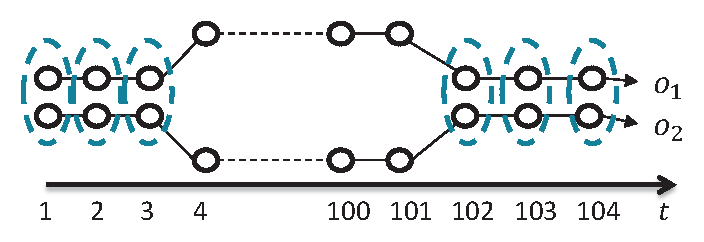
\includegraphics[width=0.5\textwidth]{platoon_weakpoint.eps}
%\caption{Miss-pattern in platoon}
%\label{fig:platoon_weakpoint}
%\end{figure}

%In platoon, a pattern for $n=2,k=4,l=2$ could be $\{o_1, o_2\}\{t_1,t_2,t_4,t_5,t_{100},t_{101}\}$. However, the snapshots $t_{100}$ and $t_{101}$ is too far away from previous snapshots. Such two snapshots are in less relation with previous snapshots and thus should be removed from the pattern. Based on this observation, we defined a \emph{generalized co-moving} pattern (as in Section~\ref{sec:definition}) to provide a more fine granular control of the pattern. In \emph{generalized co-moving} pattern, a parameter $g$ is introduce the control the \emph{maximum gap} allowed between consecutive snapshots. By so doing our generalized co-moving pattern is more expressive and can represent all the existing co-moving patterns.

%In step with the advances in localization technologies, the growth in the volume of trajectory data is rapid. Traditional single-machine methods face severe scalability problem in handling large trajectory data. For example, as reported in~\cite{li2015platoon}, a \emph{Swarm} pattern takes around 100 seconds to discover for 100k trajectories. With upto billions of trajectories in nowadays datasets, such approaches apparently become unfeasible. To tackle this challenge, we propose a  paralleled solution for discovering \emph{generalized co-moving} patterns. We then deploy our idea on the modern MapReduce platform. As our experiments show, our solution achieves well load-balance and can process billions of trajectories in XXX seconds. Several optimizations are also designed to boost our solution to be orders of magnitudes faster than baseline algorithms.

%In practice, it is cumbersome to design tailed solutions to different types of co-movement pattern discovery. 

%In reality, it is cumbersome to design tailed solutions to support 
%generality and scalability

%In this paper, our primary objectives are solving two 

As can be seen, there are various co-movement patterns requested by different applications and it is cumbersome to design a tailored solution for each type. 
%Besides, we observe that, the number of co-movement patterns could be nearly exponential. 
%For instance, in the small example in Figure~\ref{fig:related_work}, \emph{swarm} already discovers 5 patterns.
We further identify that existing patterns either miss out interesting patterns (i.e, \emph{convoy}) 
or likely contain non-interesting patterns (i.e., \emph{swarm}, \emph{platoon}).
Hence, there is a particular demand for a new pattern model to fine control the pattern result without losing expressiveness. 
The other issue with existing methods is that they are built on top of centralized indexes that are not scalable. To the best of our knowledge, the maximum number of trajectories ever evaluated is up to hundreds of thousands of trajectories. In practice, it is rather common to collect at least millions of trajectories and their scalability is left unknown. We conduct a theoretical analysis on the worst-case complexity (as listed in Table~\ref{tbl:existing_co_patterns} as well as an experimental evaluation with million-scale cardinality of a trajectory database (as shown in Figure~\ref{}). Results show that their performances degrade dramatically as the dataset size scales up and none of the existing solutions is scalable to handle large-scale trajectories.
%In fact, as shown in Table~, the mining of co-movement patterns require high complexity. For instance, the
%complexities of \emph{swarm} and \emph{platoon} are already exponential. 
%Therefore, none of them can handle millions of trajectories efficiently. 
%CAN YOU ANALYSE THEIR COMPLEXITY TO ADDRESS THE PROBLEM OF SCALABILITY.

Therefore, our primary contributions in this paper are to close these two gaps. 
First, we summarize two anomalies from existing patterns, namely, \emph{missing-pattern} and \emph{loose-connection}.
The \emph{missing-pattern}~\cite{li2010swarm} anomaly arises due to the stringent constraints on the duration of a pattern. As shown in 
Figure~\ref{fig:platoon_weakpoint} (a). if the duration size is set to be $K=4$, neither \emph{flock}s nor \emph{convoy}s
can be discovered. As we notice, object $o_1$ is temporally far from $o_2$ at timestamp $4$, which is likely to be
the result of errors in interpretation of missing points, or $o_1$ faces traffic control at time $4$. Such an anomaly can
be resolved by \emph{swarm} and \emph{platoon} due to a relaxed constraint on the duration. However, 
\emph{swarm} and \emph{platoon}'s relaxations encompass a type of non-interesting patterns which is referred
as \emph{loose-connection}~\cite{li2015platoon} anomaly. As shown in Figure~\ref{fig:platoon_weakpoint} (b),
the two objects $o_1, o_2$ 
would form a \emph{platoon} pattern $\{o_1,o_2:1,2,3, 102,103,104\}$. However, the consecutive segment on the pattern's 
duration is $98$ timestamps apart, making the co-movement behavior very weak.
%
%
%%This is because that \emph{platoon} allows the timestamps in a pattern duration to be in arbitrary distance, making the object group loosely
%connected. For instance, patterns with duration $\{1,2,100,101\}$ could be a valid \emph{platoon}; however, the two timestamps $2,100$ are too far from each other.
In reality, such a pattern is likely to be induced by periodic movements of unrelated objects such as, vehicles stopping at the same petrol station, animals pausing at the same water source etc. In current literature,
users are unable to explicitly exclude the loosely-connected patterns even when those patterns are unwanted.
%When such loosely-connected patterns are unwanted, users currently are unable to directly control the outputs.
To cope with both of the two anomalies, we propose the \emph{general co-movement pattern} 
by introducing the gap parameter $G$, which requires the distance of 
timestamps in the duration to be no larger than $G$. 
By so doing, we gain a fine-grained control over the pattern duration, which alleviates both the \emph{missing-pattern} and the \emph{loose connection} problem. Meanwhile, the general co-movement pattern does not concede its expressiveness. As we show in later sections, the general co-movement pattern is able to express existing patterns by setting appropriate parameters. Therefore, users are still able to exclude non-consecutive patterns 
or include loosely-connected patterns when they feel necessary.
%IS IT POSSIBLE TO USE FIGURE 1 TO ADDRESS THE PROBLEM OF PLATOON, INSTEAD OF PROPOSING A NEW EXAMPLE SCENARIO?

%
\begin{figure}[h]
\center
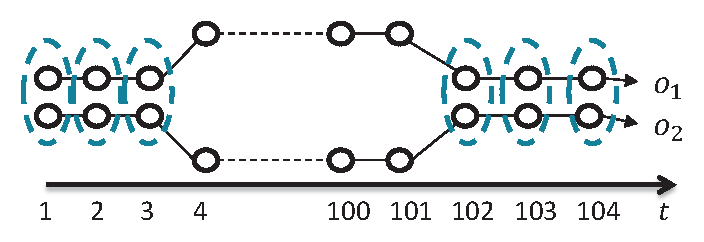
\includegraphics[width=0.4\textwidth]{platoon_weakpoint.eps}
\caption{Two anomalies in existing patterns. (a) \emph{Missing-pattern} anomaly
in \emph{flock} and \emph{convoy}. When $K=4$, none of the two patterns can be discovered. (b) \emph{Loose-connection} anomaly in \emph{platoon} and \emph{swarm}. The consecutive segment of $o_1$ and $o_2$ are 98 timestamps apart, however, the pattern $\{o_1, o_2: 1,2,3,102,103,104\}$ is included in platoon and swarm results.}
\label{fig:platoon_weakpoint}
\end{figure}
 
Second, we propose a parallel solution on modern MapReduce platforms for scalable pattern mining.
The major challenge in designing MapReduce-based algorithms is to make proper partitions of input data.
In GCMP mining, we enforce both the \emph{soundness} and the \emph{completeness} 
of the partitions. Such properties ensure that neither false-patterns 
nor miss-patterns are possible in our solution. To meet such partition requirements
as well as to keep the shuffle amount to a minimum,
% 
%%Second, we propose a . Our
%%solution is a three-step MapReduce alike approach. First, trajectories are partitioned
%%into snapshots where clusters from each snapshots are formed in parallel. Second, 
%%clusters at various timestamps are shuffled and regrouped. Third, the general co-movement patterns
%%are mined from each group. 
%
%The challenge here is to ensure that
%the patterns mined at step three is complete. If not, further shuffles and computations are required which 
%significantly drag down the system performance. In order to resolve the challenges and meanwhile keep the 
%shuffle amount at each stage to a minimum, 
we first design a naive \emph{Temporal Replication and Mining} (TRM)
approach, which partitions trajectories into groups of consecutive snapshots. Then, we design a line-sweep
method for mining GCMP from each partition. We prove that in TRM, the partition is complete and sound when a snapshot is replicated $O(|T|)$ times. 
Then, we design a novel \emph{Star Partition and Mining} (SRM) approach which significantly reduces the data shuffled
as compare to TRM. In SRM, we design a conceptual connection graph based on proximity among objects. We adapt
a \emph{star partition} which cut the graph by replicating vertices. Afterwards, we design an Apriori-like method to mine
GCMP in each partition. We prove the correctness of SPM and show that total data been replicated is $O(|\mathbb{O}|)$.
Moreover, we utilize \emph{temporal monotonicity} in GCMP to further reduce the shuffling and mining cost in SPM. Lastly, we adapt various engineering level techniques to support efficiently deploying our algorithms in 
Apache Spark which is one of the most popular MapReduce platforms.

%we design a novel star-based partition scheme to efficiently partition objects based on their
%belonging clusters. Based on the star partition, we then propose a series of optimization techniques which
%largely improve the system performance. NEED TO EMPHASIZE YOUR TECHNICAL CONTRIBUTION!

We conduct a set of extensive experiments on XXX datasets with million-scale trajectories. The results show that XXX.

The rest of our paper is organized as follows: Section~\ref{sec:related_works} summarizes the relevant literature on 
trajectory pattern mining; Section~\ref{sec:definition} forms the definition of the general co-movement pattern mining; Section~\ref{sec:system_overview} presents our parallel architecture; The solution of mining the general co-movement pattern mining is presented in Section~\ref{sec:trm_solution} and Section~\ref{sec:spm_solution}. Section~\ref{sec:optimization} discuss various optimization techniques to boost the system performance; Section~\ref{sec:experiment} conducts extensive experiments to showcase the usefulness and efficiency of our system and finally Section~\ref{sec:conclusion} concludes our paper.


